\chapter{Conclusion and summary}

This Chapter highlights the contributions, limitations and personal insights of the author in this thesis and 
proposes possible directions for future research.

\section{Main Contributions}

This thesis specifically addressed decision making by agents under uncertainty. 
In the field of Robotics and Artificial Intelligence (AI), considering uncertainty in search policies is not straightforward. 
This is due to the complexity involved in solving Partially Observable Markov Decision Processes (POMDP), 
commonly used to describe uncertainty in tasks, which become quickly infeasible for even the simplest problems. Although there has been progress in the 
development of POMDP solvers with demonstrated applications to robotics, these are predominantly verified in simulation where the action space is discretised.  

This thesis concentrates on the learning of search policies from human teachers and their transfer to a robotic apprentice,
and provides three major contributions to the current research which will be summarised below.

Firstly, we demonstrate a Programming by Demonstration POMDP framework (PbD-POMDP) to learn a mixture of search strategies 
from human teachers. We use a particle filter to represent the belief of the end-effector's position of both human teachers and the robot apprentice.
The particle filter is compressed to a belief state composed of the most likely state and entropy. 
A sequence of demonstrated belief states and actions is used to learn a generative joint belief-action distribution parameterised by 
Gaussian Mixture Model (GMM). The GMM is used as an autonomous dynamical system which gives a velocity vector field when conditioned on the current
belief state. We demonstrate that mixed behaviours, such as risk prone and adverse, are encoded by the generative model. 

Secondly, we propose a Reinforcement Learning (RL) approach to further optimise the parameters of the GMM model
to take into account the quality of the demonstrated behaviours. By introducing a binary cost function and using 
approximate dynamic programming in an actor-critic framework (which we call RL-PbD-POMDP) we are able to 
significantly improve the performance of a search strategy designed to accomplish a peg-in-hole task.
% need to say that much fewer demonstrations are needed

Thirdly, we develop a Bayesian State Space Estimator (BSSE), which we name Measurement Likelihood Memory Filter (MLMF), to solve 
the Simultaneous Localisation and Mapping (SLAM) problem where only haptic information is available. 
Given the nature of the searches, we consider any prior structure in the beliefs (such as Gaussianity) to be 
ill-suited. We demonstrate that by choosing a different parameterisation of the Histogram Bayesian filter we are able 
to overcome the inherent exponential space and time complexity. To the best of our knoweldge this is 
the first work which considers mostly negative information in a SLAM setting.

% In this thesis we demonstrate a continuous action and belief space POMDP framework for learning how to accomplish a task 
% with only haptic and proprioceptive information.

% We proposed an Programming by Demonstration method to learn a POMDP policy.

% Proposed a Reinforcement learning to improve the POMDP policy.

% We propose a method to filter the state space.

\section{Limitations and Future Work}

We summarise the current perceived limitations of our work and discuss different approaches to 
resolving them.

\subsubsection{Gaussian Mixture Controller}
%
%	-> rely on haptic information to localise oneself
%	-> non-deterministic learning process
%       -> this implies that the vector might be unadequate. 
%
Throughout this dissertation, we used Gaussian Mixture Models (GMM) to encode a vector 
field policy which is a function of the current belief state. For the robot to be able to localise 
itself the policy has to be guided towards salient areas of the state space, such as edges and corners. 
However, as the GMM learning is non-deterministic and data driven, there are no guarantees that 
behaviour such as remaining in contact with edges in order to get haptic feedback 
will be encoded and reproduced by the GMM policy. 

\begin{figure}[h]
  \centering
  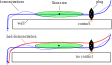
\includegraphics[width=0.9\linewidth]{./ch6-conclusion/Figures/gmm_problem.pdf}
  \caption{GMM policy drawback. \textit{Top:} Two demonstrations, blue trajectories, follow a path
  which when fitted with a GMM (one Gaussian component is drawn in green) results in a vector which keeps the plug 
  in contact with the edge of the wall. \textit{Bottom:} A third demonstration, red line, 
  did not result in a contact with the edge of the wall. The Gaussian of the GMM is shifted to the 
  mean point of the data. The GMM policy no longer keeps the plug in contact with the edge.
  }
  \label{fig:ch6:gmm_traj}
\end{figure}

It would require only one poorly demonstrated trajectory which failed to establish a contact with an edge, 
for the vector field to be shifted resulting in a policy which fails to establish
contact with the environment. Figure \ref{fig:ch6:gmm_traj} illustrates an example of this drawback.

A solution would be to design a cost function which gives more importance to data points which are close 
to salient features, such as edges and corners. As a result, the components of the problematic red trajectory in Figure 
\ref{fig:ch6:gmm_traj} are excluded during the learning. This can be integrated into the 
Actor-Critic Reinforcement Learning (RL) framework used in Chapter 4, for the peg-in-hole task.

RL is an off-line approach (in the sense that many rollouts are needed to achieve the desired behaviour) 
which can be used to select behaviour which will result in a policy remaining in contact with the environment. 
However, if the geometry of the environment was to change by less than a centimetre the same situation would occur 
(failure to remain in contact) and GMM policy parameters would have to be relearned through either new demonstrations or 
via autonomous exploration.

In the peg-in-hole task described in Chapter 4, in order to enforce a constant contact with the environment, 
a hybrid force/position controller was used which disregarded the velocity component orthonormal to the wall.
The remaining two velocity components where obtained from the GMM policy and modulated by a heuristic 
function to surmount the edges of the plug. 

The main problem arises however during the execution of the GMM policy when no sensory feedback constraints are resolved. 
Belief space planners (reviewed in Chapter 2) are approaches which take into consideration variations in the environment 
and which can produce trajectories which actively seek sensory feedback. 
These planners solve an objective function online, with contact constraints \cite{pomdp_toussain_iros_2015}.
Such online belief space planners are computationally expensive and require simulation of dynamics and sensory 
feedback in order to find an appropriate set of actions. A dynamic system approach, such as the GMM policy, 
learns the sensory-control mapping directly making it computationally cheap at runtime.

Future research could consider local adaptation of the dynamical system in order to try
and seek out specific sensory feedback. This could be achieved for instance by combining planning with 
GMM policies or learning local dynamical systems which seek out sensory feedback. The difficulty lies
in combining their joint actions.

\subsubsection{Belief compression}
%
%	Talk about the fact that we only used the mode and entropy.... does it really matter ? 
%	Is a more complicated belief necessary
%
%

Throughout this research, the belief is represented by a probability density function and the GMM policy
is learned from a dataset with a fixed number of dimensions, which is seven in our case (3 for velocity, 
3 for the most likely state and 1 for entropy). The compression of the belief to a belief state vector results 
in loss of information which weakens the Markov assumption. There exist however other compression methods, such 
as E-PCA \cite{NIPS2002_2319}. This is a non-linear dimensionality reduction technique which retrieves a set of basis probability 
distributions in order to minimise the reconstruction Kullback–Leibler (KL) divergence. 

However, such compression methods require a discretisation of the probability 
density function and then its projection to a latent space, which in the case of E-PCA, requires solving
an convex optimisation problem (iterative Newton's method) at each time step. 

Furthermore, it is also not clear what effect an improved belief compression method would have on the policy. The better 
the compression method (in terms of KL divergence) the more dimensions are necessary and as a result 
more data points will be required to train the GMM. We make the observation in both Chapter 3 and Chapter 4 that the 
GMM policy is better than a myopic policy. However, this holds true only when a large amount of uncertainty 
is present. When the uncertainty starts to decrease the Greedy method performs just as well or even better than a 
four dimensional belief state GMM. As such, it is not clear that a more sophisticated belief compression method for 
the tasks we consider would be an improvement.

%The case for using a more complicated belief compression method is hard to 
%make, when considering the difference between the GMM and myopic policy

\subsubsection{Policy representation}

% Need many Gaussian functions, many behaviour
% This would sugget that a simpler model would be required and a mismatch between 
% the original state space. 

We learned the belief space policies in task space (Cartesian position in the world's frame of reference). 
This choice entails two difficulties: the number of parameters needed to encode the task and 
generalisation.

As there is much variance in the demonstrated search behaviour (at the raw trajectory level) many parameters 
are necessary to encode the policy. The policies learned for the search tasks in this thesis required 
around 90 Gaussian functions of dimension 7. 
This is a considerable number of parameters considering the simplicity of the task (find the the table/wall, 
navigate to an edge, reach the goal). Typically more parameters also entail a poor generalisation. 

Future work could be directed towards learning a high-level policy composed of parameterised 
behaviour policies which are easily re-usable. Such policies could be parameterised by sub-goals 
and contact constraints which could be extracted by segmenting the original demonstrations.

\subsubsection{MLMF}
% 
% Draw back is that we have to discretise the marginals ? Could we use a marginal belief 
%
The Measurement Likelihood Memory Filter (MLMF), introduced in Chapter 5, is based on 
the assumption of a sparse likelihood function where mostly zero measurements are present. 
This by itself is not a weakness, but a necessary assumption to achieve a linear space complexity. 
As the time complexity remains exponential with respect to the number of objects 
(although at a lesser growth rate) we were obliged to introduce an additional independence 
assumption. This assumption implies that some information will be lost and the filtered marginals will 
be an approximate solution with respect to an optimal Bayesian filter. There is no obvious remedy 
to this problem. There are two approaches: either introduce an assumption (as we did) or perform  
an approximate evaluation of the marginalisation. An approximate marginalisation could be achieved 
by evaluating the value of the marginals at specific points and setting the remaining marginal values by interpolation.

\section{Final Words}

During my PhD I have spent a considerable amount of time studying the role 
of uncertainty in Artificial Intelligence, specifically how it affects 
decision making in agents. I list below some points of interest and important 
insights.

\begin{itemize}

 \item \textit{Humans can be poor teachers:}  Programming by Demonstration (PbD), traditionally requires an expert 
 teacher to provide a set of demonstrations in the form of state-velocity pairs which are used to learn 
 a policy represented by a regressor function. If the teacher is rarely successful at his task, learning a policy
 directly from his behaviour will yield a policy on par with the teachers performance.
 One of the original questions posed by PbD is \textit{what to imitate ?}, \cite{Billard08chapter}.
 By introducing a simple binary cost function, as shown in Chapter 4, we were able to improve the quality of the policy.
 All regression based PbD methods can use the Reinforcement Learning (RL) approach used in Chapter 4, with no additional 
 rollouts being necessary.
 
 \item \textit{Reinforcement Learning can be easy (continuous state and action space):} 
 RL is notable for needing lengthy simulations and episodes to be successful, which typically result in 
 a complete exploration of the entire state (or parameter) space for tasks
 such as the inverted-pendulum or mountain cart.  This is infeasible for learning a  complicated continuous state 
 and action space policy with a long time horizon.
 
 In using RL during both my PhD and Master Thesis, there was always some magic required
 to get RL to work, such as choosing an appropriate learning rate of the value function 
 and decay rate of the exploration noise, in order to get past local minimas. 
 
 There are two factors which make RL difficult to use: the exploration-exploitation 
 dilemma and the non-stationarity of the value function approximator during on-line learning.
 To alleviate the exploration-exploitation problem one can use human demonstrations 
 in which an optimal set of state-action pairs hopefully exists. The non-stationarity
 of the target value function can be achieved through batch methods, also known as fitted RL methods, which 
 keep all data witnessed during episodes and learn the value function off-line through 
 approximate dynamic programming. 
 Learning the value function online at each time step can lead to divergence if an appropriate 
 function approximator is not chosen \cite[p. 51]{RL_book_2010}. Given the current memory capacity 
 of modern computers the fitted RL off-line methods seem more appropriate since the RL problem
 becomes a familiar regression problem for which many algorithms are applicable.
 
 By using a fitted off-line approach to learn a value function in combination with 
 a separate parameterisation of the policy in an Actor-Critic framework, it is
 again feasible to use simple reward functions which can result in significant 
 improvements in the policy, as shown in Chapter 4.
 
  \item \textit{Myopic vs POMDP policies:} Across most of the discrete POMDP literature the Q-MDP myopic policy is 
 used as a benchmark. In the problems considered, Q-MDP does not fare as well in terms of reward but the difference 
 in the policies's parameters are not reported. Throughout this research we always used a myopic policy as a benchmark 
 to compare with our more sophisticated approaches. Even though myopic policies do not consider uncertainty when taking an action,
 the action will always lead to some information gain, since actuated robots are very precise. As a result the 
 uncertainty will always decrease and eventually the robot will manage to accomplish its task.
 It is not clear what difference exists between myopic and continuous policy search methods on point motion and 
 grasping tasks in which the uncertainty is considered uni-modal and Gaussian, as there has been no extensive comparison.
 This being said a lot depends on the perception capabilities of the robot. In an environment which provides enough
 sensory cues after a few time steps the robot will be localised regardless of the policy followed. 
\end{itemize}



% The importance of the likelihood measurement function
% 





